% Options for packages loaded elsewhere
\PassOptionsToPackage{unicode}{hyperref}
\PassOptionsToPackage{hyphens}{url}
%
\documentclass[
  man]{apa7}
\usepackage{amsmath,amssymb}
\usepackage{iftex}
\ifPDFTeX
  \usepackage[T1]{fontenc}
  \usepackage[utf8]{inputenc}
  \usepackage{textcomp} % provide euro and other symbols
\else % if luatex or xetex
  \usepackage{unicode-math} % this also loads fontspec
  \defaultfontfeatures{Scale=MatchLowercase}
  \defaultfontfeatures[\rmfamily]{Ligatures=TeX,Scale=1}
\fi
\usepackage{lmodern}
\ifPDFTeX\else
  % xetex/luatex font selection
\fi
% Use upquote if available, for straight quotes in verbatim environments
\IfFileExists{upquote.sty}{\usepackage{upquote}}{}
\IfFileExists{microtype.sty}{% use microtype if available
  \usepackage[]{microtype}
  \UseMicrotypeSet[protrusion]{basicmath} % disable protrusion for tt fonts
}{}
\makeatletter
\@ifundefined{KOMAClassName}{% if non-KOMA class
  \IfFileExists{parskip.sty}{%
    \usepackage{parskip}
  }{% else
    \setlength{\parindent}{0pt}
    \setlength{\parskip}{6pt plus 2pt minus 1pt}}
}{% if KOMA class
  \KOMAoptions{parskip=half}}
\makeatother
\usepackage{xcolor}
\usepackage{graphicx}
\makeatletter
\def\maxwidth{\ifdim\Gin@nat@width>\linewidth\linewidth\else\Gin@nat@width\fi}
\def\maxheight{\ifdim\Gin@nat@height>\textheight\textheight\else\Gin@nat@height\fi}
\makeatother
% Scale images if necessary, so that they will not overflow the page
% margins by default, and it is still possible to overwrite the defaults
% using explicit options in \includegraphics[width, height, ...]{}
\setkeys{Gin}{width=\maxwidth,height=\maxheight,keepaspectratio}
% Set default figure placement to htbp
\makeatletter
\def\fps@figure{htbp}
\makeatother
\setlength{\emergencystretch}{3em} % prevent overfull lines
\providecommand{\tightlist}{%
  \setlength{\itemsep}{0pt}\setlength{\parskip}{0pt}}
\setcounter{secnumdepth}{-\maxdimen} % remove section numbering
% Make \paragraph and \subparagraph free-standing
\ifx\paragraph\undefined\else
  \let\oldparagraph\paragraph
  \renewcommand{\paragraph}[1]{\oldparagraph{#1}\mbox{}}
\fi
\ifx\subparagraph\undefined\else
  \let\oldsubparagraph\subparagraph
  \renewcommand{\subparagraph}[1]{\oldsubparagraph{#1}\mbox{}}
\fi
\newlength{\cslhangindent}
\setlength{\cslhangindent}{1.5em}
\newlength{\csllabelwidth}
\setlength{\csllabelwidth}{3em}
\newlength{\cslentryspacingunit} % times entry-spacing
\setlength{\cslentryspacingunit}{\parskip}
\newenvironment{CSLReferences}[2] % #1 hanging-ident, #2 entry spacing
 {% don't indent paragraphs
  \setlength{\parindent}{0pt}
  % turn on hanging indent if param 1 is 1
  \ifodd #1
  \let\oldpar\par
  \def\par{\hangindent=\cslhangindent\oldpar}
  \fi
  % set entry spacing
  \setlength{\parskip}{#2\cslentryspacingunit}
 }%
 {}
\usepackage{calc}
\newcommand{\CSLBlock}[1]{#1\hfill\break}
\newcommand{\CSLLeftMargin}[1]{\parbox[t]{\csllabelwidth}{#1}}
\newcommand{\CSLRightInline}[1]{\parbox[t]{\linewidth - \csllabelwidth}{#1}\break}
\newcommand{\CSLIndent}[1]{\hspace{\cslhangindent}#1}
\ifLuaTeX
\usepackage[bidi=basic]{babel}
\else
\usepackage[bidi=default]{babel}
\fi
\babelprovide[main,import]{english}
% get rid of language-specific shorthands (see #6817):
\let\LanguageShortHands\languageshorthands
\def\languageshorthands#1{}
% Manuscript styling
\usepackage{upgreek}
\captionsetup{font=singlespacing,justification=justified}

% Table formatting
\usepackage{longtable}
\usepackage{lscape}
% \usepackage[counterclockwise]{rotating}   % Landscape page setup for large tables
\usepackage{multirow}		% Table styling
\usepackage{tabularx}		% Control Column width
\usepackage[flushleft]{threeparttable}	% Allows for three part tables with a specified notes section
\usepackage{threeparttablex}            % Lets threeparttable work with longtable

% Create new environments so endfloat can handle them
% \newenvironment{ltable}
%   {\begin{landscape}\centering\begin{threeparttable}}
%   {\end{threeparttable}\end{landscape}}
\newenvironment{lltable}{\begin{landscape}\centering\begin{ThreePartTable}}{\end{ThreePartTable}\end{landscape}}

% Enables adjusting longtable caption width to table width
% Solution found at http://golatex.de/longtable-mit-caption-so-breit-wie-die-tabelle-t15767.html
\makeatletter
\newcommand\LastLTentrywidth{1em}
\newlength\longtablewidth
\setlength{\longtablewidth}{1in}
\newcommand{\getlongtablewidth}{\begingroup \ifcsname LT@\roman{LT@tables}\endcsname \global\longtablewidth=0pt \renewcommand{\LT@entry}[2]{\global\advance\longtablewidth by ##2\relax\gdef\LastLTentrywidth{##2}}\@nameuse{LT@\roman{LT@tables}} \fi \endgroup}

% \setlength{\parindent}{0.5in}
% \setlength{\parskip}{0pt plus 0pt minus 0pt}

% Overwrite redefinition of paragraph and subparagraph by the default LaTeX template
% See https://github.com/crsh/papaja/issues/292
\makeatletter
\renewcommand{\paragraph}{\@startsection{paragraph}{4}{\parindent}%
  {0\baselineskip \@plus 0.2ex \@minus 0.2ex}%
  {-1em}%
  {\normalfont\normalsize\bfseries\itshape\typesectitle}}

\renewcommand{\subparagraph}[1]{\@startsection{subparagraph}{5}{1em}%
  {0\baselineskip \@plus 0.2ex \@minus 0.2ex}%
  {-\z@\relax}%
  {\normalfont\normalsize\itshape\hspace{\parindent}{#1}\textit{\addperi}}{\relax}}
\makeatother

\makeatletter
\usepackage{etoolbox}
\patchcmd{\maketitle}
  {\section{\normalfont\normalsize\abstractname}}
  {\section*{\normalfont\normalsize\abstractname}}
  {}{\typeout{Failed to patch abstract.}}
\patchcmd{\maketitle}
  {\section{\protect\normalfont{\@title}}}
  {\section*{\protect\normalfont{\@title}}}
  {}{\typeout{Failed to patch title.}}
\makeatother

\usepackage{xpatch}
\makeatletter
\xapptocmd\appendix
  {\xapptocmd\section
    {\addcontentsline{toc}{section}{\appendixname\ifoneappendix\else~\theappendix\fi\\: #1}}
    {}{\InnerPatchFailed}%
  }
{}{\PatchFailed}
\keywords{O*Net, challenge-hindrance framework, job demands-resources, job characteristics\newline\indent Word count: 4,942}
\DeclareDelayedFloatFlavor{ThreePartTable}{table}
\DeclareDelayedFloatFlavor{lltable}{table}
\DeclareDelayedFloatFlavor*{longtable}{table}
\makeatletter
\renewcommand{\efloat@iwrite}[1]{\immediate\expandafter\protected@write\csname efloat@post#1\endcsname{}}
\makeatother
\usepackage{csquotes}
\ifLuaTeX
  \usepackage{selnolig}  % disable illegal ligatures
\fi
\IfFileExists{bookmark.sty}{\usepackage{bookmark}}{\usepackage{hyperref}}
\IfFileExists{xurl.sty}{\usepackage{xurl}}{} % add URL line breaks if available
\urlstyle{same}
\hypersetup{
  pdftitle={Shared Characterizations of Demands and Resources across O*NET Job Elements},
  pdfauthor={Alicia Stachowski2, John Kulas1, \& Renata García Prieto Palacios Roji3},
  pdflang={en-EN},
  pdfkeywords={O*Net, challenge-hindrance framework, job demands-resources, job characteristics},
  hidelinks,
  pdfcreator={LaTeX via pandoc}}

\title{Shared Characterizations of Demands and Resources across O*NET Job Elements}
\author{Alicia Stachowski\textsuperscript{2}, John Kulas\textsuperscript{1}, \& Renata García Prieto Palacios Roji\textsuperscript{3}}
\date{}


\shorttitle{O*NET JD-R}

\authornote{

Funding: This work was supported by the College of Humanities and Social Sciences, Montclair State University, Montclair, NJ.

}

\affiliation{\vspace{0.5cm}\textsuperscript{1} eRg\\\textsuperscript{2} University of Wisconsin - Stout\\\textsuperscript{3} PepsiCo}

\abstract{%
Many discussions of job demands and resources include a tacit characterization that job elements are either resources or demands. This study documents variability in ratings of O*Net job characteristics with respect to subjective interpretation of job characteristics and predicts the form of demand (challenge or hindrance) will exhibit differential association with work--related outcomes. We additionally explore the potential moderating role of resources on these relationships. The results support the perspective that job characteristics are not uniquely categorized as a resource or demand, but rather, challenging elements tend to also be experienced as job resources. Furthermore, greater experienced resources moderated the challenge-engagement relationship as well as the hindrance-stress and hindrance-burnout relationships. These findings broadly suggest that challenging demands may also provide opportunity in the form of job resources, and what is viewed as a \emph{hindrance} exhibits considerable variability. These findings have implications for job design and management particularly with regard to opportunity with \emph{some} demanding elements: these may be candidates for growth opportunity.
}



\begin{document}
\maketitle

While we have accumulated a vast literature on how job demands and resources relate to and influence key organizational outcomes, recent work has called into question some of our basic assumptions regarding the experience of demands in particular. We build on a growing number of researchers who argue that work elements may be appraised simultaneously as resources and demands (Webster et al., 2011) or that appraisals may change over time (Rosen et al., 2020). Our primary aims explore whether: 1) variability exists in subjective ratings of job characteristics with respect to perception as resource and/or demand, 2) some characteristics are more likely than others to vary across demand and resource, 3) subjective appraisals are differentially related to positive and negative outcomes, and lastly, 4) resources buffer the relationships between demands and negative work outcomes. We investigate these associations via the lens of \href{https://www.onetcenter.org/content.html}{O*Net job specifications}, which provides a broad framework of specification regarding generalizable job characteristics.

\hypertarget{theoretical-foundations}{%
\subsection{Theoretical Foundations}\label{theoretical-foundations}}

The job demands-resources theory (e.g., Bakker \& Demerouti, 2014; 2017) highlights the importance of demands and resources on the experience of motivation and strain as well as other, less proximal outcomes. Resources include physical, psychological, social, or organizational aspects of the job that may help an employee achieve work goals, reduce job demands, or promote personal growth and development (e.g., Bakker \& Demerouti, 2014, 2017). In contrast, demands include components of a job that require sustained effort, and as such, produce psychological or physiological strain (high work pressure, for example, is commonly cited as a demand, e.g., Demerouti et al., 2001). The perception of an element of one's job as a resource or demand activates one of two distinct processes: either health impairment (resulting from demands) or motivation (resulting from resources; Bakker and Demerouti (2014)).

Cavanaugh et al. (2000) extended this orientation by proposing a framework that distinguishes between \emph{two forms} of demands -- \emph{challenges} and \emph{hindrances}. Challenge demands promote mastery, personal growth, and future gains -- these demands should lead to coping strategies that facilitate achievement. Work characteristics consistent with this definition, for example, include time pressure and responsibility (M. A. LePine, 2022). Hindrance demands, in contrast, inhibit growth, learning and goal achievement. Example hindrance demands that have been previously noted include role conflict and role ambiguity (M. A. LePine, 2022).

M. A. LePine (2022) explain the mechanisms by which demands are related to performance and wellbeing outcomes. First, demands appraised as \emph{challenges} typically result in a more positive appraisal, and engagement is likely to happen as a result. Engagement, in turn, is positively related to motivation, performance, growth, and wellbeing. Demands appraised as \emph{hindrances} elicit a different process. Disengagement is likely to result from a hindrance appraisal, which then negatively impacts motivation, performance, growth and wellbeing. This happens because resources are depleted via frustrations and other negative affect reactions (M. A. LePine, 2022).

Meta-analytic explorations of the challenge-hindrance stressor framework have generally been supportive of the framework's propositions (see, for example, J. A. LePine et al. (2005) regarding performance and Crawford et al. (2010) regarding engagement). Pindek et al. (2024) meta-analyzed diary studies of dynamic demands (i.e., short-term daily experiences of demands) and concluded that daily challenge demands had a positive \emph{direct} association with performance, but a negative \emph{indirect} association with performance through strain (as described by M. A. LePine (2022) above). As expected, hindrance demands had both direct and indirect (through strain) associations with performance (Pindek et al., 2024).

Interestingly, much of our existing knowledge regarding the way these relationships between resources/demands and outcomes (e.g., stress, engagement) function is grounded in the assumption that certain job characteristics can generally be considered to be (positive) resources while others can be considered demands. Pindek et al. (2024) notes this limitation of \emph{a priori} classification of characteristics as demands, challenges, or hindrances, as do Horan et al. (2020). In fact, although much of our research on job demands is based on \emph{a priori} classifications (Searle \& Auton, 2015), the most recent literature suggests that the classification of a work characteristic as a demand or resource is largely subjective by nature (e.g., two different employees could most certainly perceive ``delivering face--to--face presentations'' as a resource or as a demand).

Aligned with this relativistic perspective on the experience of work, Horan et al. (2020) and M. A. LePine (2022) specifically call out the need for additional research to incorporate the appraisal process into the challenge-hindrance stressor framework. In fact, Horan et al. (2020) state that ``\ldots stressors are only challenge or hindrance demands to the extent that they are perceived as such by employees'' (p.~3). They go on to suggest future research continue to move away from \emph{a priori} classifications of demands, as doing so can be problematic for theoretical and empirical reasons.

Given the above, the first question we pose is whether people exclusively experience job elements as resources, challenges, or hindrances, or whether a given job characteristic might be mutually considered as more than one of these (e.g., both a challenge and a resource). Evidence suggests that employees do, at least, differentiate between challenge and hindrance demands (e.g., Bakker \& Sanz-Vergel, 2013; Gerich, 2017; Webster et al., 2011). For example, Bakker and Sanz-Vergel (2013) found that work pressure was perceived as a hindrance, and emotional demands as more of a challenge. Webster et al. (2011) approached this question with three commonly implicated workplace demands: workload, role ambiguity, and role conflict. They found while that each could be appraised primarily as a challenge or hindrance, they could also simultaneously be perceived as being both a challenge and hindrance to different degrees. We aim to both replicate the above findings and extend them to include resources.

\begin{quote}
Hypothesis 1: Job characteristics vary regarding subjective worker perception as a challenge or hindrance demand, or resource.
\end{quote}

\begin{quote}
Hypothesis 2: Job characteristics are not exclusively categorized as a resource or demand, but rather, some job characteristics are viewed as both a resource and a demand.
\end{quote}

\hypertarget{connecting-appraisals-to-workplace-outcomes}{%
\subsection{Connecting Appraisals to Workplace Outcomes}\label{connecting-appraisals-to-workplace-outcomes}}

The second set of predictions focus on associations with theory--derived outcomes across two theoretical frameworks. Both the job demands--resources model (Bakker \& Demerouti, 2017) and the challenge-hindrance stressor framework (Cavanaugh et al., 2000) have been associated with a wide variety of organizational outcomes ranging from affective variables like job satisfaction, to motivation, commitment, and performance (e.g., J. A. LePine et al., 2005). We provide only a sampling of associated outcome examples here for context but note that the current project will focus on three outcomes: engagement, strain, and burnout. See Figure \ref{fig:ourmodel} for proposed associations, \textbf{with dotted and solid lines indicating\ldots{}} . Resources by definition include aspects of the job that may help an employee achieve work goals, reduce job demands, or promote personal growth and development (e.g., Bakker \& Demerouti, 2014, 2017), and empirical work suggests that they are associated with positive outcomes. Relevant to the current study, for example, Hakanen et al. (2008) found job resources influenced future work engagement. Moreover, in a sample of teachers and dentists, Bakker et al. (2007) found that resources were most predictive of engagement when job demands were especially high. Meta analyses have also concluded that there is a positive association with a variety of resource categories and engagement (e.g., Schaufeli, 2017).

\begin{figure}
\centering
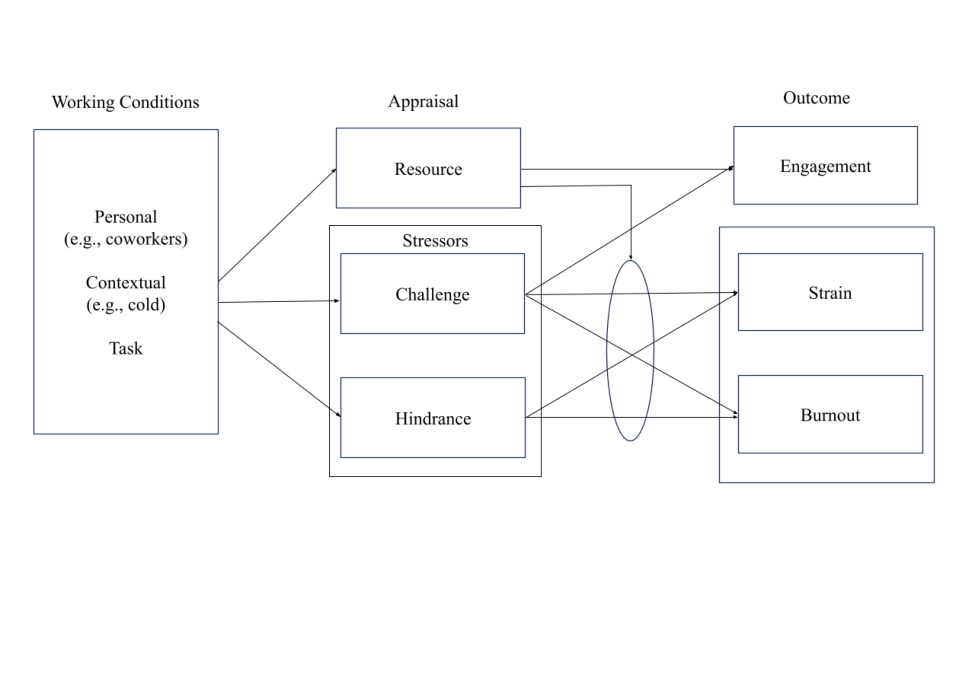
\includegraphics{Submission_files/figure-latex/ourmodel-1.pdf}
\caption{\label{fig:ourmodel}Focal constructs and associations of interest}
\end{figure}

The findings regarding demands are more complex, presumably because the way challenge vs.~hindrance appraisals influence coping strategies. Appraising a demand as a challenge has been positively associated with sources of motivation (i.e., sense of self-worth and meaningful work (Chen et al., 2021), engagement (Crawford et al., 2010), and strain and turnover intentions (e.g., Abbas \& Raja, 2019), for example. Challenge appraisals have also been negatively associated with job search behaviors (e.g., Cavanaugh et al., 2000). \textbf{CLARIFY}

When a demand is appraised as a hindrance, it is negatively associated with motivational resources (Kim \& Beehr, 2020), engagement (Crawford et al., 2010), job search behaviors and job satisfaction (Cavanaugh et al., 2000). Chen et al. (2021) found that daily hindrance demands were negatively associated with cognitive wellbeing and work family enrichment. Further, turnover intentions, turnover and withdrawal behaviors are negatively related to hindrance demands (Podsakoff et al., 2007). Interestingly, both challenges and hindrances have been shown to positively predict strain (Abbas \& Raja, 2019; J. A. LePine et al., 2005; Podsakoff et al., 2007; Webster et al., 2010), which further highlights the complex association between appraisals and subsequent outcomes. Given the differential relationships described above, we make the following predictions (see Figure \ref{fig:ourmodel}):

\begin{quote}
Hypothesis 3a: Resources and challenges positively predict engagement.
\end{quote}

\begin{quote}
Hypothesis 3b: Both challenge and hindrance demands positively predict stress and burnout.
\end{quote}

In addition to the these direct relationships, we aim to extend work suggesting that resources can act as a buffer between job demands and strain (e.g., Bakker et al., 2005) and burnout (e.g., Xanthopoulou et al., 2007). Bakker and colleagues (2005) were the first to report empirical evidence to support the idea that job resources could potentially buffer the negative impact of job demands on distal outcomes like burnout. Bakker et al. (2005) explored the interaction between 4 demands (e.g., work overload, physical demands) and 4 resources (e.g., social support, feedback) and three dimensions of burnout (exhaustion, cynicism, and professional efficacy), and found some support for the prediction that high demands with low resources predicted greater levels of cynicism and exhaustion among employees in higher education. Similarly, Xanthopoulou et al. (2007) also found some support for this interaction (high demands + low resources leads to greater burnout) among home healthcare employees. They concluded that a variety of resources, including autonomy, social support, performance feedback, and opportunities for professional development buttered the connection between demands (i.e., patient harassment, workload, physical and emotional demands) and burnout. We extend the established job demands-resources model buffer proposition to both challenge and hindrance demands as follows (see Figure \ref{fig:ourmodel}):

\begin{quote}
Hypothesis 4a:Resources moderate the relationship between challenge demands and the outcomes of strain and burnout such that these relationships become weaker as workers perceive more resources.
\end{quote}

\begin{quote}
Hypothesis 4b:Resources moderate the relationship between hindrance demands and the outcomes of strain and burnout such that these relationships become weaker as workers perceive more resources.
\end{quote}

\hypertarget{method}{%
\section{Method}\label{method}}

\hypertarget{participants}{%
\subsection{Participants}\label{participants}}

The final usable sample consisted of 568. Regarding tenure, 13.57\% had been in their referent job less than 6 months, 19.20\% between 6 months and a year, 49.12\% between one and five years, 13.27\% between 5 and 10 years, and 4.87\% more than 10 years. Respondent ages ranged from 18 to 65 with an average of 28.18 years old (\emph{SD} = 7.53). The survey offered a free-field gender identity category, although the sample predominantly self-identified as female (52.58\%) or male (46.83\%).

\hypertarget{materials}{%
\subsection{Materials}\label{materials}}

Characteristics, Challenge Demands, Hindrance Demands, and Resources. The Occupational Information Network (O*Net) serves as a repository of information broadly descriptive of occupations (Peterson et al., 2001). The O*Net database consists of hundreds of standardized and occupation-specific descriptors of occupations in the US and these descriptions are frequently updated. We focused on 98 work \href{https://www.ONETonline.org/find/descriptor/result/4.A.1.b.3}{activity and context statements} which O*Net groups into \emph{activity} categories of information input (e.g., where and how are the information and data gained that are needed to perform this job?), interacting with others (e.g., what interactions with other persons or supervisory activities occur while performing this job?), mental processes (e.g., what processing, planning, problem-solving, decision-making, and innovating activities are performed with job-relevant information?) and work output (e.g., what physical activities are performed, what equipment and vehicles are operated/controlled, and what complex/technical activities are accomplished as job outputs?). Work \emph{context} statements are grouped into interpersonal relationships (e.g., the context of the job in terms of human interaction processes), physical work conditions (e.g., the work context as it relates to the interactions between the worker and the physical job environment), and structural job characteristics (e.g., the relationships or interactions between the worker and the structural characteristics of the job).

O*Net collects information about these categories by periodically asking workers job characteristic questions, which often have \href{https://www.ONETonline.org/find/descriptor/result/4.C.1.c.2}{unique response categories}. For example, ``How responsible is the worker for work outcomes and results of other workers?'' has response options ranging from \emph{no responsibility} to \emph{very high responsibility}, while the question, ``How often do you use electronic mail in this job?'' has options ranging from \emph{never} to \emph{every day}. We retained O*Net's response scales while asking for statement relevance, all of which shared the same 5-point scale regardless of semantic label difference. Other than minor grammatical editing (for example, changing ``the worker'' to ``you''), we also retained the O*Net wording for our item stems. The total number of items on each administered survey was less than 392 (98 characteristics x 4 repeated measurements) because we did not ask for demand and resource evaluations for 14 O*Net characteristics that we projected would have very low frequency of endorsement across respondents (one excluded characteristic, for example, was \emph{\ldots the extent to which the worker is exposed to radiation on the job}).

Participants were asked to think about whether or not their job could be described as consisting of 98 different O*Net job characteristics. For example, if a respondent indicated that any one characteristic was not applicable for their job (e.g., answered \emph{never} or \emph{not at all}), they were not subsequently asked to rate the level of resource (\ldots this aspect of your job is a resource that can be functional in achieving work goals, reduce job demands, or stimulate personal growth/development), challenge (\ldots this aspect of your job is a challenge that can promote mastery, personal growth, or future gains), or hindrance (\ldots this aspect of your job is a hindrance that can inhibit personal growth, learning, and work goal attainment) in randomized order. Participants were compensated six USD for their participation (the estimated time commitment pre-administration was 45 minutes).

Stress. Stress was captured via three items taken from the Copenhagen Psychosocial Questionnaire (Burr et al., 2019). Responses were provided using a Likert-type scale ranging from (1) Not at All to (5) All the Time. A sample item is, ``How often have you had problems relaxing because of your job?''. Obtained alpha was .85 in this sample.

Burnout. Four items from the Copenhagen Psychosocial Questionnaire (Burr et al., 2019) were used to assess burnout. Again, responses were provided using a Likert-type scale ranging from (1) Not at All to (5) All the Time. A sample item is, ``How often have you felt worn out?''. Alpha was 0.85 in this sample.

Engagement. The 18-item engagement measure was recently developed (Russell et al., 2022), with the authors specifying three subscales which yielded current sample 𝛼's of
0.68 (absorption) and 0.80 (vigor), and 0.90 (dedication). Responses were provided using a Likert-type scale ranging from (1) Strongly Disagree to (6) Strongly Agree. A sample item is, ``I enjoy thinking about work even when I'm not at work''. For the purposes of the current study, we focused on an overall engagement score (18 item aggregate, α = 0.91).

\hypertarget{procedure}{%
\subsection{Procedure}\label{procedure}}

Data were collected through Prolific, an online data collection platform. An email was sent to eligible members of the Prolific respondent pool, notifying them of their opportunity to participate. Eligibility requirements included being 18 or older and holding either a full-time or part-time job. Eligible individuals then voluntarily chose whether or not to respond to the invitation after reading an informed consent.

Respondents were asked to think about their primary job, and each administered survey branched content dependent on whether or not the respondent's job could be described as consisting of 98 different O*Net job characteristics in randomized order. Participants were compensated six USD for their participation (the estimated time commitment pre-administration was 45 minutes). See Figure \ref{fig:onetviz} for a visual representation of the process experienced by respondents.

\begin{figure}
\centering
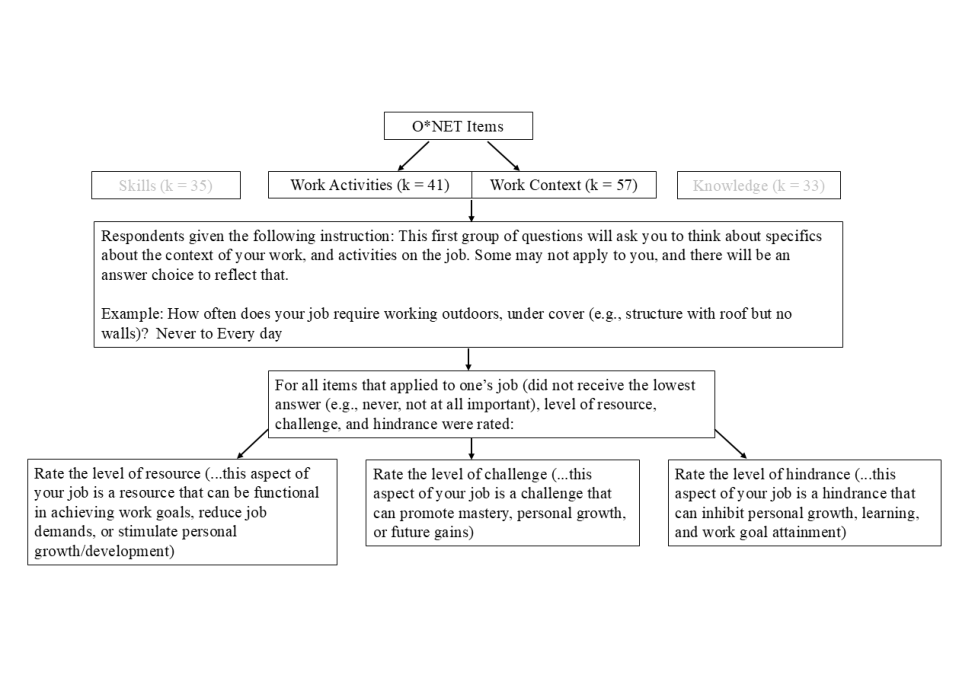
\includegraphics{Submission_files/figure-latex/onetviz-1.pdf}
\caption{\label{fig:onetviz}Visual representation of how respondents experienced the survey.}
\end{figure}

\hypertarget{results}{%
\section{Results}\label{results}}

Of the 785 individuals who initially accessed the survey link, 112 indicated that they were not interested, had more than 200 missing responses, or had 20 or more identical consecutive sequential responses (Yentes \& Wilhelm, 2021). Applying a further screen regarding attention checks (there were four attention checks embedded throughout, asking respondents to indicate a specific answer) resulted in the retention of 568 respondents who constitute the current sample.

\begin{figure}
\centering
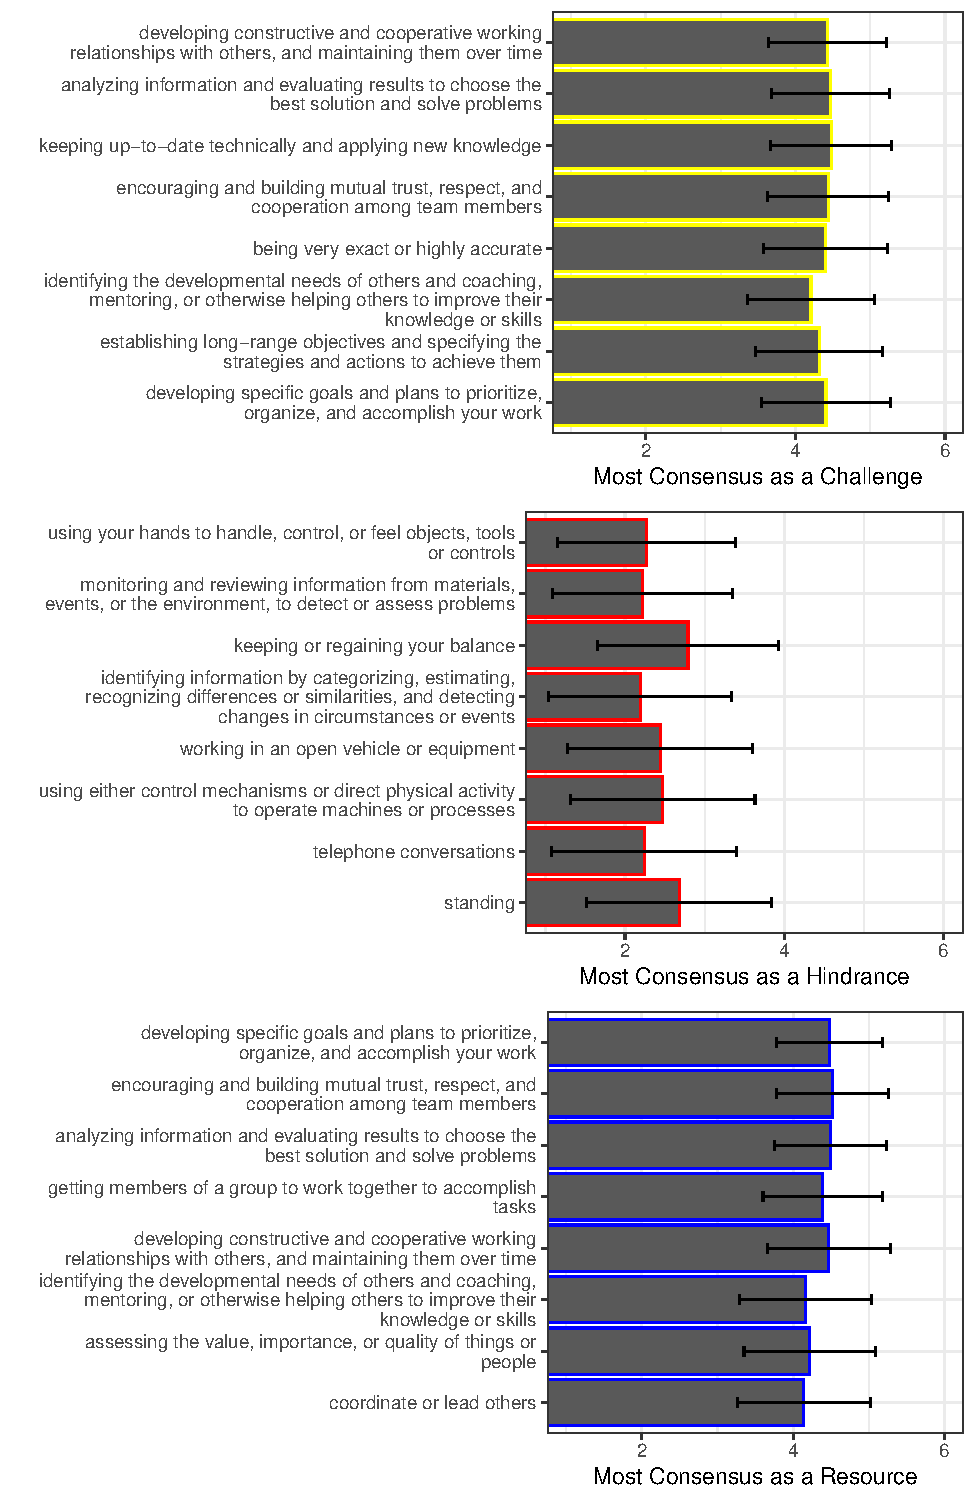
\includegraphics{Submission_files/figure-latex/combinegraphs-1.pdf}
\caption{\label{fig:combinegraphs}Characteristics percieved most similarly (lowest standard deviations).}
\end{figure}

\begin{figure}
\centering
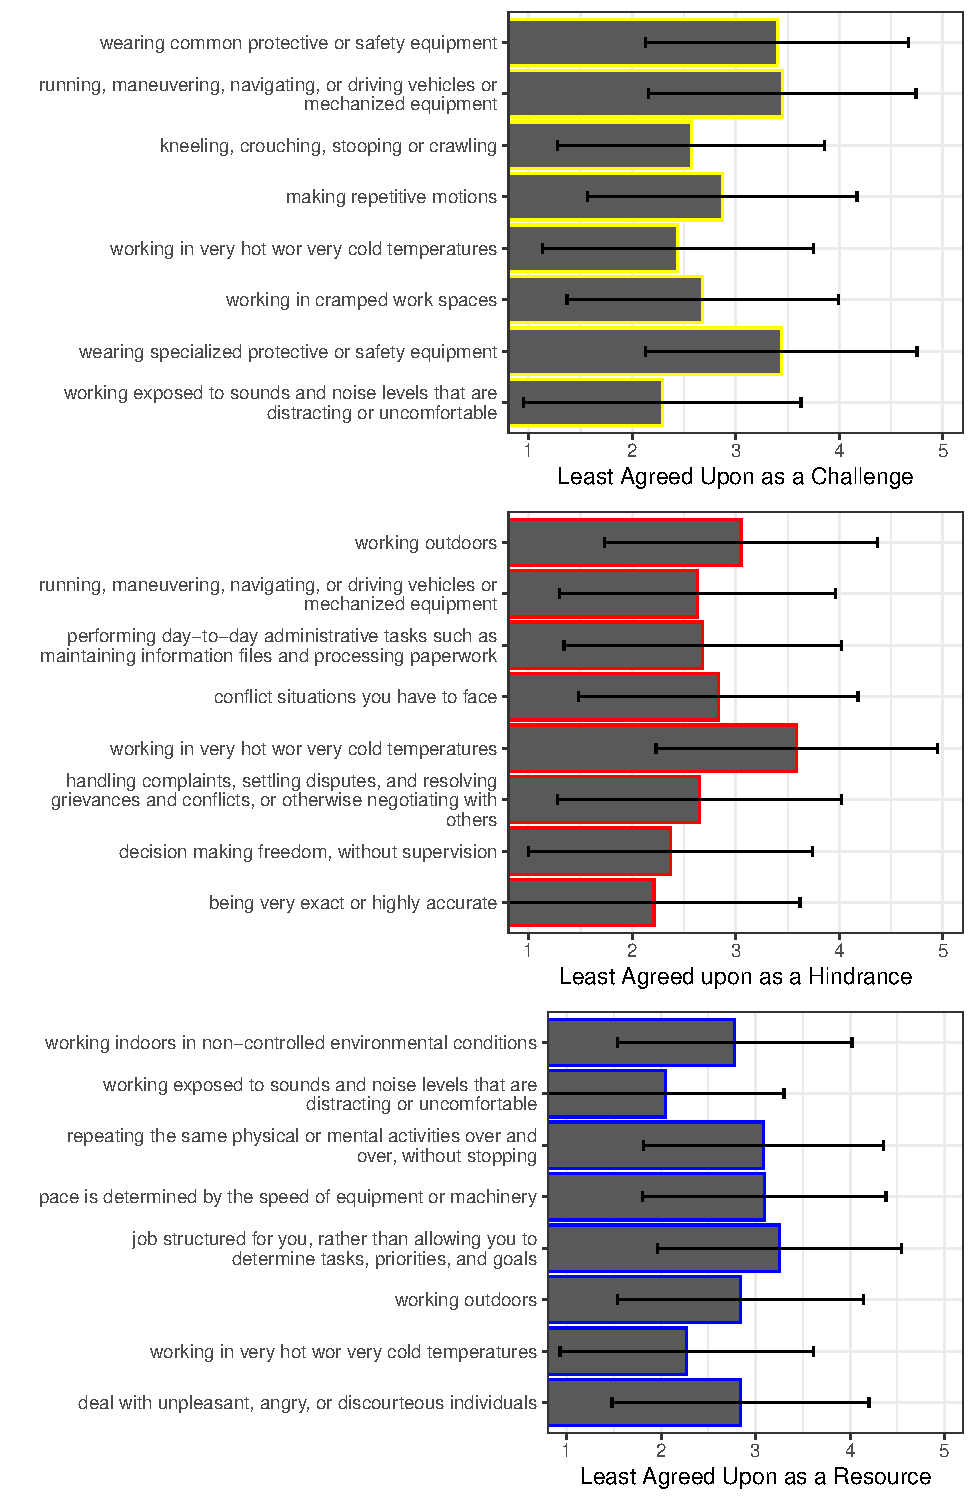
\includegraphics{Submission_files/figure-latex/combinegraphs2-1.pdf}
\caption{\label{fig:combinegraphs2}Characteristics percieved most \textbf{dissimilarly} (largest standard deviations).}
\end{figure}

\begin{figure}
\centering
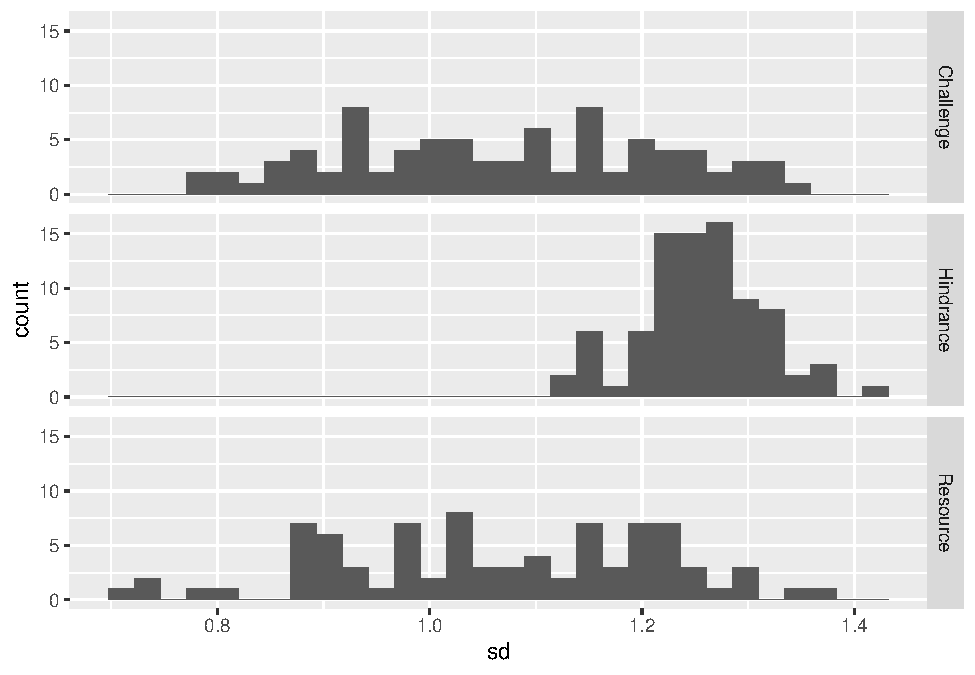
\includegraphics{Submission_files/figure-latex/overallhist-1.pdf}
\caption{\label{fig:overallhist}Frequency distribution of standard deviations across characteristics deemed resources, challenges, and demands.}
\end{figure}

H1 posits that static job characteristics are not necessarily always experienced similarly across workers - as hindrances, challenges, or resources. We explore this hypothesis first at the job characteristic level before presenting a broader perspective. Figures \ref{fig:combinegraphs} and \ref{fig:combinegraphs2} present only extreme snapshots of characteristic variability in the form of the 8-most \emph{consistently rated} and \emph{inconsistently rated} resources, challenges, and demands.\footnote{A full list of item characteristic ratings, along with summary averages and standard deviations is available in supplementary online resources. The Figures \ref{fig:combinegraphs} and \ref{fig:combinegraphs2} presentations are only limited to 8 characteristics per perceived category because of space restrictions (there are 252 individual characteristic ratings in the online resources).} These figures present average item ratings, but the central elements of interest are the standard deviations, which reflect the characteristics with the relative most and least consistency. Figure \ref{fig:combinegraphs} presents the resources, challenges, and hindrances that are \emph{most consistently agreed on} as indexed by (relatively) low standard deviations, while Figure \ref{fig:combinegraphs2} presents the characteristics with the greatest amount of \emph{disagreement} across workers. The figures demonstrate that what is perceived as resource and challenge tends to be somewhat agreed upon (the range of the ``lowest 8'' resource standard deviations is 0.70 to 0.88 and the range of lowest 8 challenge standard deviations is 0.79 to 0.86). However, there is considerably less relative agreement regarding the degree to which job elements should be considered to be hindrances, with the 8 elements showing the \emph{greatest agreement} still ranging in fairly large standard deviations (ranging from 1.12 to 1.16).

In addition to highlighting extremely agreed- or disagreed-upon characteristics, Figure \ref{fig:overallhist} presents our standard deviation indices across all rated items. Here, discrepancies receive greater context, with the \emph{spread} of difference exhibiting wider distributions of agreement for challenge and resource ratings (and relatively \emph{bunched} levels of disagreement for hindrances; note the spread of the challenge and resource histograms relative to the hindrance histogram). Some characteristics are largely agreed upon as being challenges and resources, while all hindrance perceptions exhibit a relatively higher level of disagreement. This points to \emph{hindrances}, in particular, as being likely amenable to future probing regarding moderating conditions. A Bartlett's test for homogeneity of variance across the challenge, hindrance, and resource ratings confirms this difference (\(\chi^2_{}\) = 76.83, \emph{p} \textless{} .01). In sum, these results provide some collective support for H1, and particularly so for hindrances, which are differently experienced across our raters.

The second hypothesis stated that job characteristics would not be uniquely categorized as a resource or demand. Table 1 provides the correlations among the O*Net ``scale''-level groupings across ratings of resource, challenge, and hindrance (i.e., Information Input (ii), Mental Processes (mp), Work Output (wo), Interacting with Others (io), Interpersonal Relationships (ir), Physical Work Conditions (pc), and Structural Job Characteristics (sc)). We would expect to see minimal correlations if job characteristics \emph{were} uniquely categorized. First, the average correlation within all resource categories (variables 1 through 7 in Table 1) was .43 (\emph{SD} = .13, range from .15 to .64), and challenge categories exhibited similar associations (ranging from .12 to .70, \emph{M} = .43, \emph{SD} =.16). Hindrance categories, however, had less differentiation across categories, with relatively elevated correlations ranging from .33 to .86, \emph{M} = .62, \emph{SD} = .17. When people perceived hindrances, these seem to be shared across different types of job activities, whereas challenges and resources exhibit greater differentiation.

The mean resource to challenge correlations within the same dimension ranged from .62 to .66 (\emph{M} = .64, \emph{SD} = .02; for example, the association between information input ratings as a resource and as a challenge was .62). The correlations between resources and challenges \emph{across} dimensions (for example, the correlation between mental processes and work output was .42 and .39) ranged from .08 to .50, \emph{M} = .32, \emph{SD} = .12. The resource-hindrance correlations within the same dimension ranged from -.16 to -.30 (\emph{M} = -.24, \emph{SD} = .05), while the correlations between resources and hindrances \emph{across} dimensions ranged from .05 to -.27, \emph{M} = -.14, \emph{SD} = .08. The mean challenge to hindrance correlations within the same dimension ranged from -.04 to -.27 (\emph{M} = -.21, \emph{SD} = .08). The correlations between challenges to hindrances across dimensions ranged from .12 to -.26, \emph{M} = -.11, \emph{SD} = .09. In summary, correlations were larger when what was being rated was the same type of characteristic. Challenge and hindrance demands demonstrated smaller relationships, but mostly negative. Challenges and resources within the same O*Net dimensions are strongly and positively related. These results provide support for H2, suggesting that there is overlap in how employees perceive job characteristics - particularly regarding what is perceived as a \emph{resource} being also perceived as a \emph{challenge}. Stated another way, job characteristics are not uniquely categorized as a resource or as a demand.

The next group of hypotheses focuses on the relationship among resources and demands (challenge and hindrance) and outcomes. Table 2 shows the overall associations between resource/challenge/hindrances and outcomes of engagement, stress, and burnout. Here, we observe positive associations between resources, and challenges with engagement, and a negative association between hindrances and engagement. A positive association is observed between hindrances and stress.

\begin{lltable}

\begin{TableNotes}[para]
\normalsize{\textit{Note.} $*$ p < .05, $**$ p < .01; The seven O*Net grouping categories represented here are: Information Input (ii), Mental Processes (mp), Work Output (wo), Interacting with Others (io), Interpersonal Relationships (ir), Physical Work Conditions (pc), and Structural Job Characteristics (sc)}
\end{TableNotes}

\tiny{

\begin{longtable}{m{2.6cm}m{.7cm}m{.7cm}m{.7cm}m{.7cm}m{.7cm}m{.7cm}m{.7cm}m{.7cm}m{.7cm}m{.7cm}m{.7cm}m{.7cm}m{.7cm}m{.7cm}m{.7cm}m{.7cm}m{.7cm}m{.7cm}m{.7cm}m{.7cm}}\noalign{\getlongtablewidth\global\LTcapwidth=\longtablewidth}
\caption{\label{tab:cortab}Challenge, hindrance, and resource bivariate correlations.}\\
\toprule
 & \multicolumn{1}{c}{1} & \multicolumn{1}{c}{2} & \multicolumn{1}{c}{3} & \multicolumn{1}{c}{4} & \multicolumn{1}{c}{5} & \multicolumn{1}{c}{6} & \multicolumn{1}{c}{7} & \multicolumn{1}{c}{8} & \multicolumn{1}{c}{9} & \multicolumn{1}{c}{10} & \multicolumn{1}{c}{11} & \multicolumn{1}{c}{12} & \multicolumn{1}{c}{13} & \multicolumn{1}{c}{14} & \multicolumn{1}{c}{15} & \multicolumn{1}{c}{16} & \multicolumn{1}{c}{17} & \multicolumn{1}{c}{18} & \multicolumn{1}{c}{19} & \multicolumn{1}{c}{20}\\
\midrule
\endfirsthead
\caption*{\normalfont{Table \ref{tab:cortab} continued}}\\
\toprule
 & \multicolumn{1}{c}{1} & \multicolumn{1}{c}{2} & \multicolumn{1}{c}{3} & \multicolumn{1}{c}{4} & \multicolumn{1}{c}{5} & \multicolumn{1}{c}{6} & \multicolumn{1}{c}{7} & \multicolumn{1}{c}{8} & \multicolumn{1}{c}{9} & \multicolumn{1}{c}{10} & \multicolumn{1}{c}{11} & \multicolumn{1}{c}{12} & \multicolumn{1}{c}{13} & \multicolumn{1}{c}{14} & \multicolumn{1}{c}{15} & \multicolumn{1}{c}{16} & \multicolumn{1}{c}{17} & \multicolumn{1}{c}{18} & \multicolumn{1}{c}{19} & \multicolumn{1}{c}{20}\\
\midrule
\endhead
1. onet.resource.ii & - &  &  &  &  &  &  &  &  &  &  &  &  &  &  &  &  &  &  & \\
2. onet.resource.mp & .61** & - &  &  &  &  &  &  &  &  &  &  &  &  &  &  &  &  &  & \\
3. onet.resource.wo & .46** & .50** & - &  &  &  &  &  &  &  &  &  &  &  &  &  &  &  &  & \\
4. onet.resource.io & .49** & .64** & .45** & - &  &  &  &  &  &  &  &  &  &  &  &  &  &  &  & \\
5. onet.resource.ir & .46** & .55** & .37** & .60** & - &  &  &  &  &  &  &  &  &  &  &  &  &  &  & \\
6. onet.resource.pc & .19** & .15** & .32** & .18** & .37** & - &  &  &  &  &  &  &  &  &  &  &  &  &  & \\
7. onet.resource.sc & .43** & .46** & .41** & .45** & .48** & .37** & - &  &  &  &  &  &  &  &  &  &  &  &  & \\
8. onet.challenge.ii & .62** & .49** & .37** & .41** & .33** & .08 & .33** & - &  &  &  &  &  &  &  &  &  &  &  & \\
9. onet.challenge.mp & .47** & .63** & .42** & .50** & .41** & .09* & .38** & .65** & - &  &  &  &  &  &  &  &  &  &  & \\
10. onet.challenge.wo & .34** & .39** & .64** & .34** & .30** & .29** & .38** & .45** & .49** & - &  &  &  &  &  &  &  &  &  & \\
11. onet.challenge.io & .34** & .48** & .33** & .65** & .48** & .13** & .40** & .50** & .68** & .43** & - &  &  &  &  &  &  &  &  & \\
12. onet.challenge.ir & .32** & .40** & .26** & .48** & .63** & .23** & .39** & .46** & .60** & .39** & .70** & - &  &  &  &  &  &  &  & \\
13. onet.challenge.pc & .12** & .08 & .21** & .13** & .26** & .66** & .29** & .14** & .12** & .33** & .20** & .31** & - &  &  &  &  &  &  & \\
14. onet.challenge.sc & .27** & .31** & .28** & .38** & .40** & .27** & .62** & .36** & .41** & .38** & .51** & .45** & .40** & - &  &  &  &  &  & \\
15. onet.hindrance.ii & -.26** & -.26** & -.17** & -.24** & -.18** & -.02 & -.08 & -.27** & -.26** & -.10* & -.19** & -.16** & .06 & -.10* & - &  &  &  &  & \\
16. onet.hindrance.mp & -.23** & -.30** & -.17** & -.22** & -.15** & .05 & -.07 & -.22** & -.27** & -.10* & -.18** & -.15** & .12** & -.06 & .86** & - &  &  &  & \\
17. onet.hindrance.wo & -.21** & -.25** & -.22** & -.22** & -.06 & -.02 & -.12** & -.14** & -.21** & -.23** & -.15** & -.09* & .05 & -.10* & .66** & .69** & - &  &  & \\
18. onet.hindrance.io & -.22** & -.27** & -.14** & -.29** & -.18** & -.01 & -.10* & -.21** & -.25** & -.10* & -.27** & -.19** & .07 & -.10* & .79** & .86** & .69** & - &  & \\
19. onet.hindrance.ir & -.22** & -.24** & -.15** & -.24** & -.25** & -.06 & -.11** & -.19** & -.21** & -.08* & -.20** & -.23** & .04 & -.12** & .79** & .80** & .61** & .82** & - & \\
20. onet.hindrance.pc & -.04 & -.08* & -.09* & -.11** & -.10* & -.16** & -.13** & -.03 & -.04 & -.06 & -.08* & -.10* & -.04 & -.13** & .38** & .33** & .47** & .35** & .47** & -\\
21. onet.hindrance.sc & -.13** & -.15** & -.13** & -.19** & -.13** & -.09* & -.23** & -.12** & -.10* & -.05 & -.16** & -.12** & -.01 & -.17** & .62** & .62** & .56** & .64** & .66** & .45**\\
\bottomrule
\addlinespace
\insertTableNotes
\end{longtable}

}

\end{lltable}

\begin{table}[tbp]

\begin{center}
\begin{threeparttable}

\caption{\label{tab:unnamed-chunk-1}Overall variable bivariate correlations.}

\begin{tabular}{llllllll}
\toprule
 & \multicolumn{1}{c}{1} & \multicolumn{1}{c}{2} & \multicolumn{1}{c}{3} & \multicolumn{1}{c}{4} & \multicolumn{1}{c}{5} & \multicolumn{1}{c}{$M$} & \multicolumn{1}{c}{$SD$}\\
\midrule
1. Challenge & - &  &  &  &  & 3.75 & 0.50\\
2. Hindrance & -.21*** & - &  &  &  & 2.39 & 0.78\\
3. Resource & .74*** & -.25*** & - &  &  & 3.77 & 0.48\\
4. Stress & -.03 & .11** & -.08 & - &  & 2.59 & 0.97\\
5. Burnout & -.05 & .08 & -.08 & .70*** & - & 3.04 & 0.87\\
6. Engagement & .28*** & -.11** & .33*** & -.24*** & -.30*** & 4.03 & 0.79\\
\bottomrule
\addlinespace
\end{tabular}

\begin{tablenotes}[para]
\normalsize{\textit{Note.} $*$ p < .05, $**$ p < .01, $***$ p < .001}
\end{tablenotes}

\end{threeparttable}
\end{center}

\end{table}

\hypertarget{challenges-resources-and-outcomes}{%
\subsubsection{Challenges, Resources, and Outcomes}\label{challenges-resources-and-outcomes}}

\begin{table}[tbp]

\begin{center}
\begin{threeparttable}

\caption{\label{tab:chal-resource-table}Moderated regression summary of outcomes regressed on challenges and resources}

\begin{tabular}{llllll}
\toprule
DV & \multicolumn{1}{c}{Step} & \multicolumn{1}{c}{Model} & \multicolumn{1}{c}{$\beta$} & \multicolumn{1}{c}{$R^2$} & \multicolumn{1}{c}{$\Delta R^2$}\\
\midrule
Engagement & 1 & Challenge & -0.08 &  & \\
 &  & Resource & 0.37 ** & 0.15 ** & \\
 & 2 & Challenge & 0.12 &  & \\
 &  & Resource & 0.57 ** &  & \\
 &  & Challenge X Resource & -0.4 * & 0.16 ** & 0.01 *\\
Stress & 1 & Challenge & 0.12 &  & \\
 &  & Resource & -0.06 & 0.01 & \\
 & 2 & Challenge & 0.08 &  & \\
 &  & Resource & -0.1 &  & \\
 &  & Challenge X Resource & 0.09 & 0.01 & 0.00\\
Burnout & 1 & Challenge & 0.28 ** &  & \\
 &  & Resource & -0.12 & 0.04 ** & \\
 & 2 & Challenge & 0.13 ** &  & \\
 &  & Resource & -0.26 &  & \\
 &  & Challenge X Resource & 0.29 & 0.04 ** & 0.00\\
\bottomrule
\addlinespace
\end{tabular}

\begin{tablenotes}[para]
\normalsize{\textit{Note.} * = p < .05; ** = p < .01, coefficients are unstandardized}
\end{tablenotes}

\end{threeparttable}
\end{center}

\end{table}

H3a predicted that both resources and challenges would predict engagement. Table \ref{tab:chal-resource-table} summarizes the results for engagement (as well as stress and burnout). Sum scores for the predictors were used here such that the overall amount of resource or demand is recognized. First, challenges and resources explained a statistically significant amount of the variability in engagement, \(R^2\) = 0.15, Adj. \(R^2\) = 0.15, \(F(2, 565) = 50.09\), \(p < .001\). Here, the resource slope is significant, wheras the challenge slope is not significant (providing partial support for H3a). The inclusion of the interaction term in step two of the model contributed a significant addition to the model, \(F(3, 564) = 35.62\), \(p < .001\), \(\Delta R^2\) = 0.01, \(\Delta F\) (1, 564) = 5.82, and thus provides statistical support for the presence of moderation (Hypothesis 4a). Figure \ref{fig:chal-resource-int} illustrates the interaction. With low levels of resources, the relationship between challenges and engagement is relatively flat and engagement is comparatively low. With more resources, the relationship between challenges and engagement is negative, but engagement still remains higher with greater reported challenge when more resources are perceived.

Next, challenge demands and resources did not explain a significant amount of the variance in stress, \(R^2\) = 0.01, Adj. \(R^2\) = 0, \(F(2, 565) = 1.67\), \(p = .189\), failing to provide support for Hypothesis 3b. The inclusion of the interaction term in step two of the model did not contribute a significant addition to the model, \(F(3, 564) = 1.17\), \(p = .320\), \(\Delta R^2\) = 0.00, \(\Delta F\) (1, 564) = 0.17, and thus does not support the presence of moderation.

Finally, challenge demands and resources explained a statistically significant amount of the variability in burnout, \(R^2\) = 0.04, Adj. \(R^2\) = 0.04, \(F(2, 565) = 1.67\), \(p = .189\). The inclusion of the interaction term in step two of the model did not contribute a significant addition to the model, \(F(3, 564) = 1.17\), \(p = .320\), \(\Delta R^2\) = 0.00, \(\Delta F\) (1, 564) = 2.25, and thus failing to provide statistical support for the presence of moderation (Hypothesis 4a). In sum, these findings do not provide support for the assertion that resources would moderate the relationships between challenge demands and the outcomes of strain and burnout.

\begin{table}[tbp]

\begin{center}
\begin{threeparttable}

\caption{\label{tab:hind-resource-table}Moderated regression summary of outcomes regressed on hindrances and resources}

\begin{tabular}{llllll}
\toprule
DV & \multicolumn{1}{c}{Step} & \multicolumn{1}{c}{Model} & \multicolumn{1}{c}{$\beta$} & \multicolumn{1}{c}{$R^2$} & \multicolumn{1}{c}{$\Delta R^2$}\\
\midrule
Engagement & 1 & Hindrance & -0.11 ** &  & \\
 &  & Resource & 0.35 ** & 0.17 ** & \\
 & 2 & Hindrance & -0.07 ** &  & \\
 &  & Resource & 0.37 ** &  & \\
 &  & Hindrance X Resource & -0.06 & 0.17 ** & 0.00\\
Stress & 1 & Hindrance & 0.08 * &  & \\
 &  & Resource & 0.01 & 0.01 * & \\
 & 2 & Hindrance & 0.66 ** &  & \\
 &  & Resource & 0.30 &  & \\
 &  & Hindrance X Resource & -0.77 ** & 0.04 ** & 0.03 **\\
Burnout & 1 & Hindrance & 0.09 * &  & \\
 &  & Resource & 0.10 * & 0.04 ** & \\
 & 2 & Hindrance & 0.46 * &  & \\
 &  & Resource & 0.29 &  & \\
 &  & Hindrance X Resource & -0.5 ** & 0.05 ** & 0.01 **\\
\bottomrule
\addlinespace
\end{tabular}

\begin{tablenotes}[para]
\normalsize{\textit{Note.} * = p < .05; ** = p < .01, coefficients are unstandardized}
\end{tablenotes}

\end{threeparttable}
\end{center}

\end{table}

\hypertarget{hindrances-resources-and-outcomes}{%
\subsubsection{Hindrances, Resources, and Outcomes}\label{hindrances-resources-and-outcomes}}

We also explored whether there was an interaction between hindrance demands and resources on the outcome variables. Sum scores for the predictors were used here again. First, hindrance demands and resources explained a statistically significant amount of the variability in engagement, \(R^2\) = 0.17, Adj. \(R^2\) = 0.16, \(F(2, 565) = 55.90\), \(p < .001\) {[}see Table \ref{tab:hind-resource-table}{]}. The inclusion of the interaction term in step two of the model did not contribute a significant addition to the model, \(F(3, 564) = 37.25\), \(p < .001\), \(\Delta R^2\) = 0.00, \(\Delta F\) (1, 564) = 0.13. An interaction between hindrances and resources was not found.

Next exploring stress, hindrance demands and resources explained a statistically significant amount of the variability in stress, \(R^2\) = 0.01, Adj. \(R^2\) = 0.01, \(F(2, 565) = 3.13\), \(p = .045\). The inclusion of the interaction term in step two of the model contributed a significant addition to the model, \(F(3, 564) = 6.89\), \(p < .001\), \(\Delta R^2\) = 0.03, \(\Delta F\) (1, 564) = 14.28, supporting the presence of a moderated effect. See Figure \ref{fig:hind-resource-stress-int}. As expected, the relationship between hindrance demands and strain becomes weaker as workers perceive more resources.

Similarly, hindrance demands and resources explained a statistically significant amount of the variability in burnout, \(R^2\) = 0.04, Adj. \(R^2\) = 0.03, \(F(2, 565) = 10.68\), \(p < .001\). The inclusion of the interaction term in step two of the model contributed a significant addition to the model, \(F(3, 564) = 9.49\), \(p < .001\), \(\Delta R^2\) = 0.01, \(\Delta F\) (1, 564) = 6.89, supporting the presence of a moderated effect (see Figure \ref{fig:hind-resource-burn-int}). As expected, the relationship between hindrance demands and burnout becomes weaker as workers perceive more resources. Summatively these findings provide support for the assertion that resources would moderate the relationships between hindrance demands and the outcomes of strain and burnout.

\begin{figure}
\centering
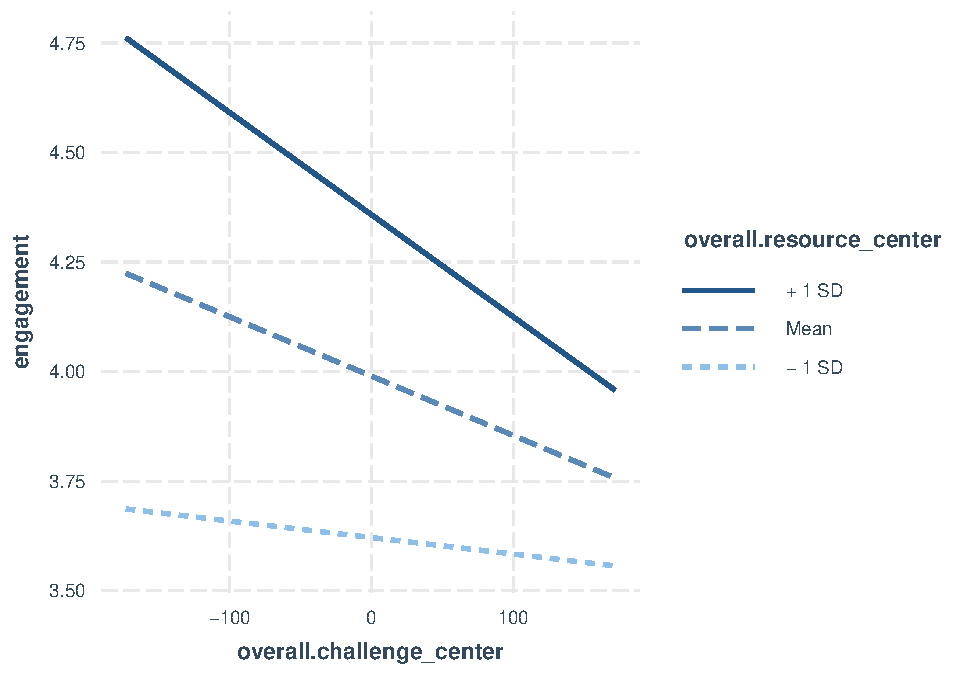
\includegraphics{Submission_files/figure-latex/chal-resource-int-1.pdf}
\caption{\label{fig:chal-resource-int}Interaction between Challenge and Resources on Engagement}
\end{figure}

\begin{figure}
\centering
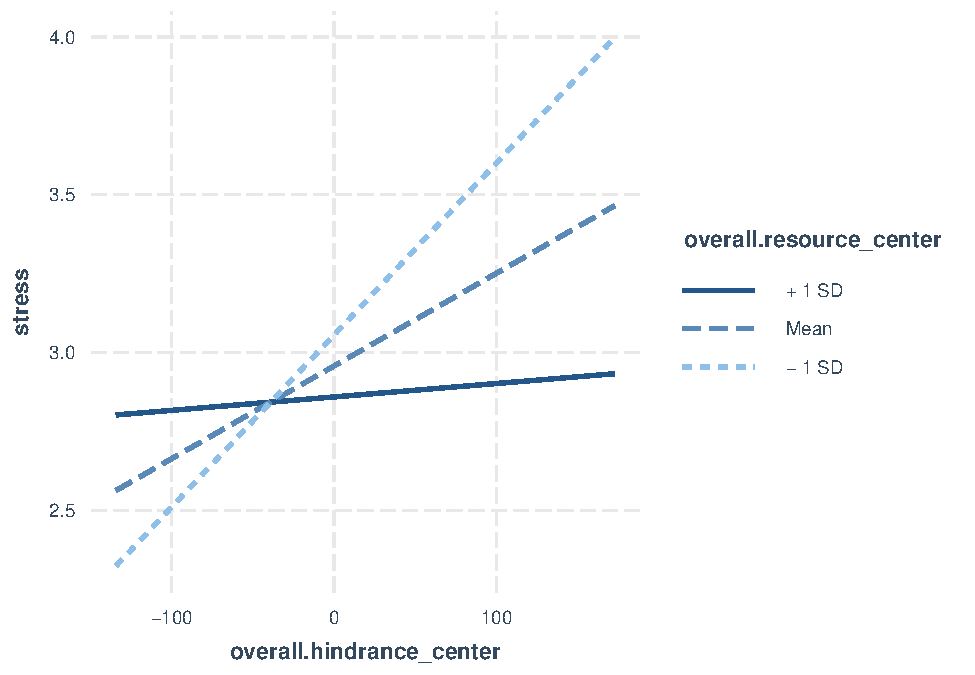
\includegraphics{Submission_files/figure-latex/hind-resource-stress-int-1.pdf}
\caption{\label{fig:hind-resource-stress-int}Interaction between Hindrances and Resources on Stress}
\end{figure}

\begin{figure}
\centering
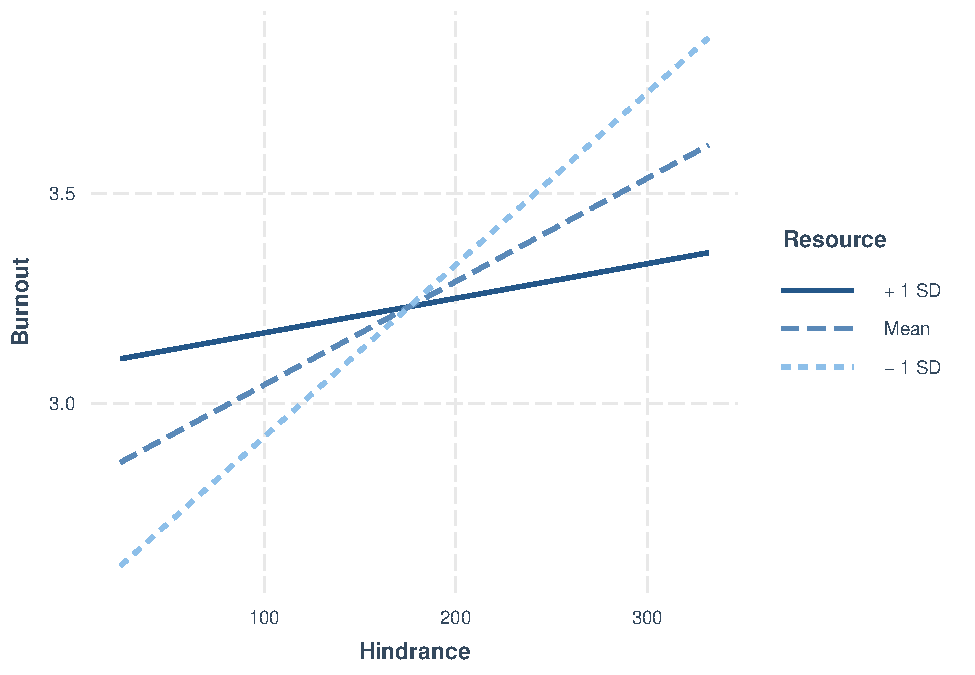
\includegraphics{Submission_files/figure-latex/hind-resource-burn-int-1.pdf}
\caption{\label{fig:hind-resource-burn-int}Interaction between Hindrances and Resources on Burnout}
\end{figure}

\hypertarget{discussion}{%
\section{Discussion}\label{discussion}}

The major aims of this paper were to explore whether: 1) there was variability in subjective ratings of job characteristics as resources and demands, 2) some characteristics were more likely to vary across demand and resource, 3) subjective appraisals were differentially related to positive and negative outcomes, and lastly, 4) if resources buffer the relationships between demands (challenge and hindrance) and outcomes. We found that job characteristics were not uniquely categorized as a resource or demand, but rather, some job characteristics were rated highly as both a resource and a demand (particularly challenge demands). The findings broadly revealed that there was relatively more consistency in ratings of resource and challenge characteristics, and far more variability in job characteristics rated as hindrance demands. This finding lends additional evidence to Horan et al. (2020)'s conclusion that ``\ldots stressors are only challenge or hindrance stressors to the extent that they are perceived as such by employees'' (p.~3). While we did not find support for the prediction that different types of demands would be related to stress and burnout, we did find that resources moderated the challenge-engagement relationship, and further, resources moderated the hindrance-stress, and hindrance-burnout relationships (as predicted).

In addition to the above findings, this paper made several additional important contributions. We utilized a diverse sample of employees across industries who responded to common O*Net items. While O*Net provides detailed information about frequency and importance ratings among employees, we begin the process of expanding what we know of job characteristics to ratings of an extensive range of demands and resources. Further, we provide a repository for other researchers with listing of O*Net demands and resources across activity and context items for the benefit of all future researchers. We also explored not only context and activity holistically, but at a higher level aggregation, which enhances our knowledge of how employees perceive different categories of resources, challenges, and hindrances within different work dimensions, as well as the relationships among them.

\hypertarget{implications}{%
\subsection{Implications}\label{implications}}

The findings presented above have implications for both theory and practice. our findings support the related literature suggesting that perceptions of resources and demands, broadly, are not universal - there are individual differences in how employees experience the characteristics of their jobs (Webster et al., 2011). This finding aligns quite well with the challenge-hindrance stressor framework, which collectively argue that employees perceive stimuli (i.e., job characteristics) uniquely (Lazarus \& Folkman, 1984), and thus, could appraise them as either a challenge or hindrance to their job performance (Cavanaugh et al., 2000). Further, Cavanaugh et al. (2000) suggests that challenge demands are typically associated with positive outcomes and hindrance demands are associated with negative outcomes (e.g., Cavanaugh et al., 2000), which we partially supported here.

Our results suggest that what is generally seen as a resource and challenge tends to be agreed upon more so that what is seen a hindrance. In fact, hindrance demands are rated more variably and thus, it may be important to have conversations about job characteristics and expectations at multiple time points after hire. For example, having open conversations with employees regarding their subjective perceptions of characteristics that may be unique in limiting their performance or comfort. Such conversations could happen during an annual performance review. In addition, J. A. LePine et al. (2005) and Podsakoff et al. (2007) encourage organizations to incorporate strain-reducing activities like training and support to offset the negative effects of challenging job demands, which may be associated with increased performance in the short term, but strain when prolonged. The current results suggest that these activities and training sessions would ideally be personalized.

Resources did predict engagement, and did moderate several of the challenge-outcome, and hindrance-outcome relationships. As such, we provide further evidence of the importance of perceived resources, particularly when a job is high in hindrance demands, as resources acted as a buffer in both instances. It is worth noting that this paper focused on \emph{perceived} resources, challenges, and hindrances. Differences in outcomes depending on whether or not an employee perceives a job characteristic to be a challenge or hindrance have practical implications especially for managers. Helping employees to manage expectations and frame the work is quite likely to shape how activities are appraised (e.g., as a challenge, or as a resource). Of course, in some instances, framing an activity or job context variable as an opportunity or positive aspect of work is unrealistic, and so interventions aimed at supporting employees (e.g., stress interventions) may be necessary.

\hypertarget{limitations-and-future-directions}{%
\subsection{Limitations and Future Directions}\label{limitations-and-future-directions}}

As with all individual studies, this project was limited in scope, and as such, there are a number of avenues for future study worth exploring. First, although we aggregated to O*Net groupings, we were also dealing with single-item measures for much our operationalization. Although not ideal psychometrically, this provided a strong linkage to the established O*Net framework. Related to that, we intentionally worked within the O*Net database, and in selecting job context and activity items, did not include other types of job characteristics that may be important resources and demands. Therefore, to the extent that O*Net is not an exhaustive repository, there are existing characteristics that we did not capture. For example, O*Net also includes styles and values, which we did not sample. Future studies may want to expand to explore these additional aspects of work.

We also retained the literature-derived definitions of resources, challenges, and hindrances (Demerouti et al., 2001). Given the high associations observed between ratings of resource and challenge, it is possible that respondents did not distinguish between these definitions as cleanly as we intended. Future investigations may wish to explore the colloquial versus academic phrasing of these questions and how that may impact observed associations between resources and challenges. We also note that effect sizes were small and thus it is important to consider the practical significance when thinking about potential interventions. We encourage future thought on how consideration of resource and demand perceptions might be combined with moderators to reduce employee stress and burnout, as well as enhance engagement.

Another interesting avenue for future research is to explore these patterns by job type. Kubicek et al. (2023), for instance, found that employee workload was positively related to strain, and that this relationship was stronger for care and social workers compared to other types of employees. This finding suggests that job type may be an important moderator, and worthy of exploration moving forward.

Lastly, there may be some practical utility to pursue training interventions aimed at \emph{how} characteristics are appraised. Perhaps the clinical literature may be informative - for example, within cognitive behavioral therapeutic applications, the way in which situations are appraised can be a mechanism to help battle affective disorders such as depression. Given the current findings, where the same characteristic may be viewed similarly as both a demand and resource, it is possible that framing interventions may ameliorate negative outcomes of demands such as, for example, stress or strain.

\hypertarget{conclusion}{%
\subsection{Conclusion}\label{conclusion}}

In sum, this endeavor builds on the challenge-hindrance stressor literature from a unique lens from within a universally accessible framework. We showed that there are far more individual differences in how employees perceive demands and resources than much of our current research suggests. While resources and challenges were more similarly experienced, what is experienced as a hindrance tends to be more variable. We further provide additional evidence highlighting the value of perceived resources in the workplace, as they were demonstrated to moderate both challenge-engagement, and hindrance-stress/hindrance burnout relationships.

\hypertarget{references}{%
\section{References}\label{references}}

\begingroup
\setlength{\parindent}{-0.5in}
\setlength{\leftskip}{0.5in}

\hypertarget{refs}{}
\begin{CSLReferences}{1}{0}
\leavevmode\vadjust pre{\hypertarget{ref-abbas2019challenge}{}}%
Abbas, M., \& Raja, U. (2019). Challenge-hindrance stressors and job outcomes: The moderating role of conscientiousness. \emph{Journal of Business and Psychology}, \emph{34}(2), 189--201.

\leavevmode\vadjust pre{\hypertarget{ref-bakker2014job}{}}%
Bakker, A. B., \& Demerouti, E. (2014). Job demands--resources theory. \emph{Wellbeing: A Complete Reference Guide}, 1--28.

\leavevmode\vadjust pre{\hypertarget{ref-bakker2017job}{}}%
Bakker, A. B., \& Demerouti, E. (2017). Job demands--resources theory: Taking stock and looking forward. \emph{Journal of Occupational Health Psychology}, \emph{22}(3), 273.

\leavevmode\vadjust pre{\hypertarget{ref-bakker2005job}{}}%
Bakker, A. B., Demerouti, E., \& Euwema, M. C. (2005). Job resources buffer the impact of job demands on burnout. \emph{Journal of Occupational Health Psychology}, \emph{10}(2), 170.

\leavevmode\vadjust pre{\hypertarget{ref-bakker2007job}{}}%
Bakker, A. B., Hakanen, J. J., Demerouti, E., \& Xanthopoulou, D. (2007). Job resources boost work engagement, particularly when job demands are high. \emph{Journal of Educational Psychology}, \emph{99}(2), 274.

\leavevmode\vadjust pre{\hypertarget{ref-bakker2013weekly}{}}%
Bakker, A. B., \& Sanz-Vergel, A. I. (2013). Weekly work engagement and flourishing: The role of hindrance and challenge job demands. \emph{Journal of Vocational Behavior}, \emph{83}(3), 397--409.

\leavevmode\vadjust pre{\hypertarget{ref-cavanaugh2000empirical}{}}%
Cavanaugh, M. A., Boswell, W. R., Roehling, M. V., \& Boudreau, J. W. (2000). An empirical examination of self-reported work stress among US managers. \emph{Journal of Applied Psychology}, \emph{85}(1), 65.

\leavevmode\vadjust pre{\hypertarget{ref-chen2021daily}{}}%
Chen, H., Wang, H., Yuan, M., \& Xu, S. (2021). Daily challenge/hindrance demands and cognitive wellbeing: A multilevel moderated mediation model. \emph{Frontiers in Psychology}, \emph{12}, 616002.

\leavevmode\vadjust pre{\hypertarget{ref-crawford2010linking}{}}%
Crawford, E. R., LePine, J. A., \& Rich, B. L. (2010). Linking job demands and resources to employee engagement and burnout: A theoretical extension and meta-analytic test. \emph{Journal of Applied Psychology}, \emph{95}(5), 834.

\leavevmode\vadjust pre{\hypertarget{ref-demerouti2001job}{}}%
Demerouti, E., Bakker, A. B., Nachreiner, F., \& Schaufeli, W. B. (2001). The job demands-resources model of burnout. \emph{Journal of Applied Psychology}, \emph{86}(3), 499.

\leavevmode\vadjust pre{\hypertarget{ref-gerich2017relevance}{}}%
Gerich, J. (2017). The relevance of challenge and hindrance appraisals of working conditions for employees' health. \emph{International Journal of Stress Management}, \emph{24}(3), 270.

\leavevmode\vadjust pre{\hypertarget{ref-hakanen2008job}{}}%
Hakanen, J. J., Schaufeli, W. B., \& Ahola, K. (2008). The job demands-resources model: A three-year cross-lagged study of burnout, depression, commitment, and work engagement. \emph{Work \& Stress}, \emph{22}(3), 224--241.

\leavevmode\vadjust pre{\hypertarget{ref-horan2020review}{}}%
Horan, K. A., Nakahara, W. H., DiStaso, M. J., \& Jex, S. M. (2020). A review of the challenge-hindrance stress model: Recent advances, expanded paradigms, and recommendations for future research. \emph{Frontiers in Psychology}, \emph{11}, 560346.

\leavevmode\vadjust pre{\hypertarget{ref-kim2020thriving}{}}%
Kim, M., \& Beehr, T. A. (2020). Thriving on demand: Challenging work results in employee flourishing through appraisals and resources. \emph{International Journal of Stress Management}, \emph{27}(2), 111.

\leavevmode\vadjust pre{\hypertarget{ref-kubicek2023all}{}}%
Kubicek, B., Uhlig, L., Hülsheger, U. R., Korunka, C., \& Prem, R. (2023). Are all challenge stressors beneficial for learning? A meta-analytical assessment of differential effects of workload and cognitive demands. \emph{Work \& Stress}, \emph{37}(3), 269--298.

\leavevmode\vadjust pre{\hypertarget{ref-lazarus1984stress}{}}%
Lazarus, R. S., \& Folkman, S. (1984). \emph{Stress, appraisal, and coping}. Springer publishing company.

\leavevmode\vadjust pre{\hypertarget{ref-lepine2005meta}{}}%
LePine, J. A., Podsakoff, N. P., \& LePine, M. A. (2005). A meta-analytic test of the challenge stressor--hindrance stressor framework: An explanation for inconsistent relationships among stressors and performance. \emph{Academy of Management Journal}, \emph{48}(5), 764--775.

\leavevmode\vadjust pre{\hypertarget{ref-lepine2022challenge}{}}%
LePine, M. A. (2022). The challenge-hindrance stressor framework: An integrative conceptual review and path forward. \emph{Group \& Organization Management}, \emph{47}(2), 223--254.

\leavevmode\vadjust pre{\hypertarget{ref-peterson2001understanding}{}}%
Peterson, N. G., Mumford, M. D., Borman, W. C., Jeanneret, P. R., Fleishman, E. A., Levin, K. Y., Campion, M. A., Mayfield, M. S., Morgeson, F. P., Pearlman, K., et al. (2001). Understanding work using the occupational information network (o* NET): Implications for practice and research. \emph{Personnel Psychology}, \emph{54}(2), 451--492.

\leavevmode\vadjust pre{\hypertarget{ref-pindek2024dynamic}{}}%
Pindek, S., Meyer, K., Valvo, A., \& Arvan, M. (2024). A dynamic view of the challenge-hindrance stressor framework: A meta-analysis of daily diary studies. \emph{Journal of Business and Psychology}, 1--19.

\leavevmode\vadjust pre{\hypertarget{ref-podsakoff2007differential}{}}%
Podsakoff, N. P., LePine, J. A., \& LePine, M. A. (2007). Differential challenge stressor-hindrance stressor relationships with job attitudes, turnover intentions, turnover, and withdrawal behavior: A meta-analysis. \emph{Journal of Applied Psychology}, \emph{92}(2), 438.

\leavevmode\vadjust pre{\hypertarget{ref-rosen2020challenges}{}}%
Rosen, C. C., Dimotakis, N., Cole, M. S., Taylor, S. G., Simon, L. S., Smith, T. A., \& Reina, C. S. (2020). When challenges hinder: An investigation of when and how challenge stressors impact employee outcomes. \emph{Journal of Applied Psychology}, \emph{105}(10), 1181.

\leavevmode\vadjust pre{\hypertarget{ref-schaufeli2017applying}{}}%
Schaufeli, W. B. (2017). Applying the job demands-resources model: A `how to'guide to measuring and tackling work engagement and burnout. \emph{Organizational Dynamics}, \emph{46}(2), 120--132.

\leavevmode\vadjust pre{\hypertarget{ref-searle2015merits}{}}%
Searle, B. J., \& Auton, J. C. (2015). The merits of measuring challenge and hindrance appraisals. \emph{Anxiety, Stress, \& Coping}, \emph{28}(2), 121--143.

\leavevmode\vadjust pre{\hypertarget{ref-webster2010toward}{}}%
Webster, J. R., Beehr, T. A., \& Christiansen, N. D. (2010). Toward a better understanding of the effects of hindrance and challenge stressors on work behavior. \emph{Journal of Vocational Behavior}, \emph{76}(1), 68--77.

\leavevmode\vadjust pre{\hypertarget{ref-webster2011extending}{}}%
Webster, J. R., Beehr, T. A., \& Love, K. (2011). Extending the challenge-hindrance model of occupational stress: The role of appraisal. \emph{Journal of Vocational Behavior}, \emph{79}(2), 505--516.

\leavevmode\vadjust pre{\hypertarget{ref-xanthopoulou2007job}{}}%
Xanthopoulou, D., Bakker, A. B., Dollard, M. F., Demerouti, E., Schaufeli, W. B., Taris, T. W., \& Schreurs, P. J. (2007). When do job demands particularly predict burnout? The moderating role of job resources. \emph{Journal of Managerial Psychology}, \emph{22}(8), 766--786.

\leavevmode\vadjust pre{\hypertarget{ref-R-careless}{}}%
Yentes, R. D., \& Wilhelm, F. (2021). \emph{Careless: Procedures for computing indices of careless responding}.

\end{CSLReferences}

\endgroup


\end{document}
